\chapter{Calibrating an optical tracking system}
\section{Assignment 3.1}
\textbf{Read and understand the papers from Zhang and Heikkil (provided in LEA). Based on your understanding of camera calibration, design a calibration setup and detail the actual calibration process. \\
Test the provided camera on your laptop and ensure you can capture still images.}

\begin{itemize}
\item We used VLC player as a tool to capture images since we can disable the auto-focussing function that is in-built in the camera with VLC player. This is required since auto-focussing changes the focal length of the lens changes. Resolution of images taken is 1280 x 800.
\end{itemize}

\section{Deliverables 3.1}
\textbf{Write a design report describing the calibration process, including a theoretical part that describes the camera and lens errors measured and corrected by the calibration. Your design report should cover:}

\subsection{A description of the setup for calibration, including possible pitfalls}

\begin{figure}[H]
\begin{center}
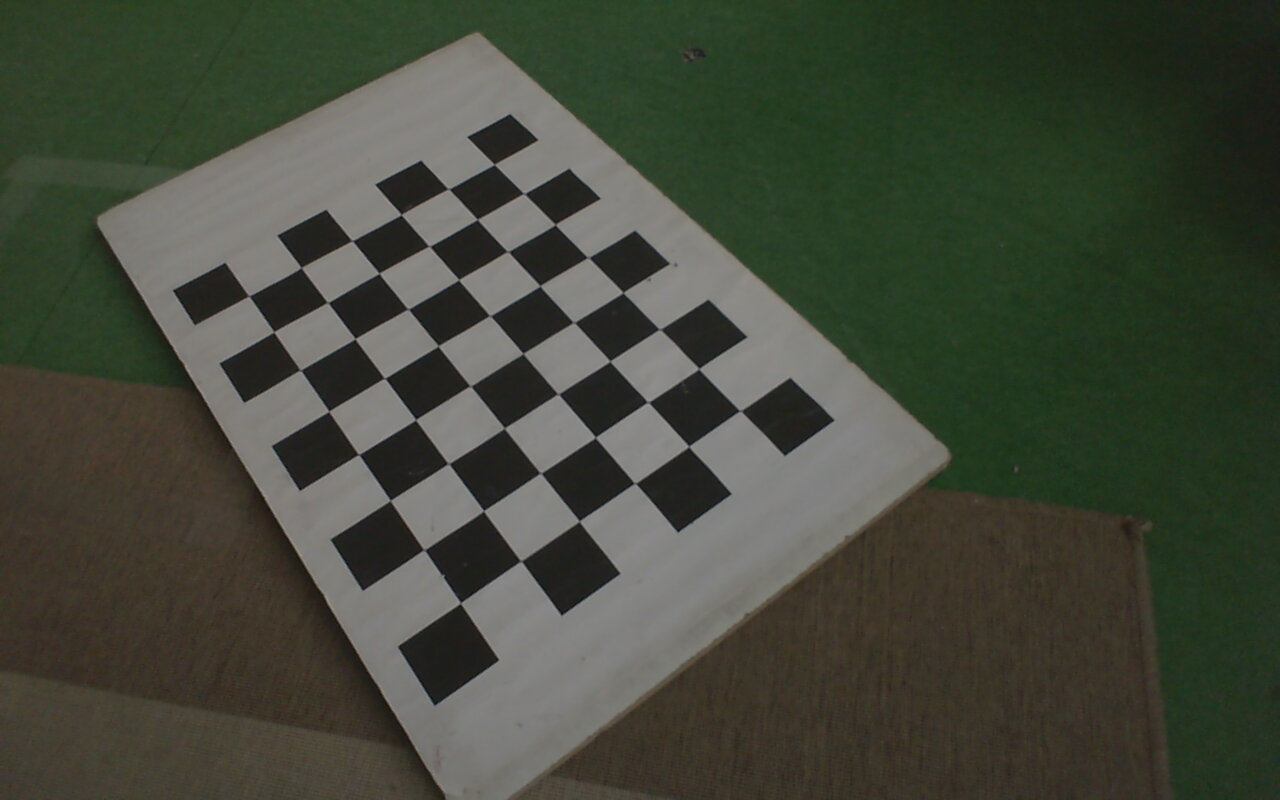
\includegraphics[width=0.6\textwidth]{data/1.jpg}
\caption{Sample image}
\label{fig:sample}
\end{center}
\end{figure}

\begin{itemize}
\item As shown in fig. \ref{fig:sample}, we place the checker board on the ground.
\item The checker board must not be square.
\item The size of the checker board was measured to be $72$ mm.
\item The provided camera is then used to take images of this checker board from multiple perspectives.
\item The poses for each image captured can be found in fig. \ref{fig:poses}.
\end{itemize}

\subsection{An estimation of the number of images and image positions required}
\begin{itemize}
\item The \texttt{Camera Calibrator} in \texttt{MatLab} required at least 3 images for calibration.
\item It is recommended that we use at least 10-20 images for calibration so that the optimization function can converge efficiently.
\item We used 51 images. This introduces a lot of redundancy however it enables us to attain higher calibration accuracy.
\item The camera's resolution is 1280 * 800
\end{itemize}

\subsection{A description of the parameters (what do they mean?) calculated by the Matlab calibration toolbox}
The standard camera model calibration algorithm assumes a pinhole camera model:
\begin{equation}
w \begin{bmatrix} x & y & 1 \end{bmatrix} = \begin{bmatrix} X & Y & Z & 1 \end{bmatrix} \begin{bmatrix} R \\ t \end{bmatrix} K
\end{equation}
where,
\begin{itemize}
\item $(X,Y,Z)$ are world coordinates of a point.
\item $(x,y)$ are image coordinates of the corresponding image point in pixels.
\item $w$ is arbitrary homogeneous coordinates scale factor.
\item $K$ is the camera intrinsic matrix defined as
\begin{equation}
K = \begin{bmatrix}
f_x & 0 & 0 \\
s & f_y & 0 \\
c_x & c_y & 1
\end{bmatrix}
\end{equation} 
\begin{itemize}
\item The coordinates $(c_x, c_y)$ represent the optical center (principal point) in pixels.
\item When $x$- and $y$-axes are orthogonal to each other, the skew parameter $s$ equals $0$.
\item $f_x = F*s_x$
\item $f_y = F*s_y$
\item $F$ is the focal length in world units, typically expressed in millimeters.
\item $[s_x, s_y]$  are the number of pixels per world unit in the x and y direction respectively.
\item $f_x$ and $f_y$ are expressed in pixels.
\end{itemize}
\item $R$ rotation matrix represents the 3D rotations of the camera.
\item $t$ represents the translation of the camera relative to the world coordinate system.
\end{itemize}


\newpage
\textbf{Distortions:}


Because lenses refract light in several cascaded lenses, distortion happens as it is shown in Figure \ref{fig:calibrationradialdistortion}. 
In order to counteract distortion Matlab's camera model can be extended with radial distortion coefficients, which are defined as follows:

\begin{equation}
x_{r\_distorted} = x(1 + k_1*r^2 + k_2*r^4 + k_3*r^6
\end{equation}
\begin{equation}
y_{r\_distorted} = y(1 + k_1*r^2 + k_2*r^4 + k_3*r^6)
\end{equation}

with:

x,y = coordinates of undistorted pixels

k = Radial distortion coefficients of the lens

$r^n = x^n + y^n$

\begin{figure}[H]
	\centering
	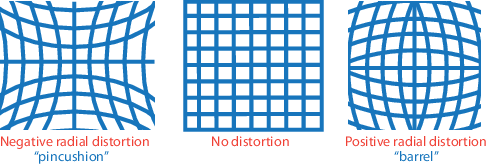
\includegraphics[width=0.5\linewidth]{graphics/calibration_radial_distortion}
	\caption[]{Types of distortion}
	
	\label{fig:calibrationradialdistortion}
\end{figure}



Since the calibration board and the camera are usually not precisely aligned some tangential distortion is introduced. This is depicted in \ref{fig:calibrationtangentialdistortion}. In the left half there is an example of a properly aligned setup, while a not aligned setup is shown on the right side.

\begin{equation}
x_{t\_distorted} = x + [2 * p_1 * x * y + p_2 * (r^2 + 2 * x^2)]
\end{equation}
\begin{equation}
yt_{t\_distorted} = y + [p_1 * (r^2 + 2 *y^2) + 2 * p_2 * x * y]
\end{equation}


with:

x,y = coordinates of undistorted pixels

k = Radial distortion coefficients of the lens

$r^n = x^n + y^n$

\begin{figure}[H]
	\centering
	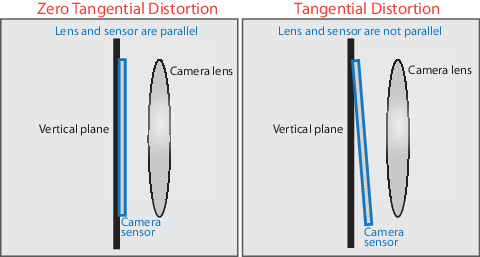
\includegraphics[width=0.5\linewidth]{graphics/calibration_tangentialdistortion}
	\caption{Tangential distortion}
	\label{fig:calibrationtangentialdistortion}
\end{figure}


\subsection{Discuss possible problems or error sources that can disturb the calibration process. Include any observation you may have made while testing the proper functioning of the camera with your laptop}
\begin{itemize}
\item We observed that unsteady setup could introduce blur in the image. Such images are bad examples to use for calibration procedure.
\item Some devices, like the provided camera, came with built-in auto-focussing function. This is undesirable since auto-focussing changes the focal length of the lens. We cannot use pin-hole camera model for cameras with variable focal length.
\end{itemize}



\section{Assignment 3.2}
\subsection*{Perform the camera calibration experiment designed in assignment 3.1. Document all relevant aspects needed to assess the quality of your obtained camera parameters.}

	

\begin{itemize}
	
\item The intrinsic camera matrix was evaluated to be:
\begin{equation}
K = 10^3\begin{bmatrix}
1.0018 & 0 & 0 \\
0.0028 & 1.0066 & 0 \\
0.6217 & 0.4154 & 0.0010
\end{bmatrix}
\end{equation}
\item The radial distortion was computed to be 
\begin{equation}
\begin{bmatrix}
0.0087 & 0.0619 & -0.1739
\end{bmatrix}
\end{equation}
\item The tangential distortion was computed to be 
\begin{equation}
\begin{bmatrix}
0.0029 & -6.6483 \cdot 10^{-4}
\end{bmatrix}
\end{equation}
\end{itemize}

\section{Deliverables 3.2}
\textbf{Write a report describing the calibration process, including a theoretical part that describes the camera and lens errors measured and corrected by the calibration:}
\subsection*{1. Describe the images poses used for calibration and report the found camera parameters including any error estimates (where applicable)}
For the camera calibration we stuck to the process outlined by Matlab, as presented in \ref{fig:cameracalibratorappsteps}

\begin{figure}[ht!]
	\centering
	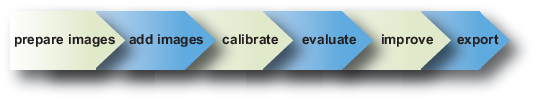
\includegraphics[width=0.7\linewidth]{graphics/cameracalibrator_app_steps}
	\caption{Steps used in camera calibration}
	\label{fig:cameracalibratorappsteps}
\end{figure}

The various image poses estimated via the calibration procedure is shown in fig. \ref{fig:poses}.
\begin{figure}[H]
\begin{center}
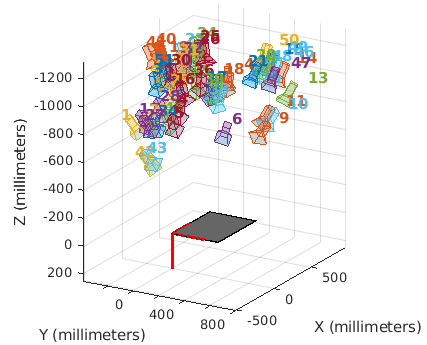
\includegraphics[width=0.7\textwidth]{graphics/camera_positions.png}
\caption{Camera positions evaluated via calibration procedure.}
\label{fig:poses}
\end{center}
\end{figure}

The example of the worst reprojection error is shown in fig. \ref{fig:worst-calibrated-image}.
\begin{figure}[H]
\begin{center}
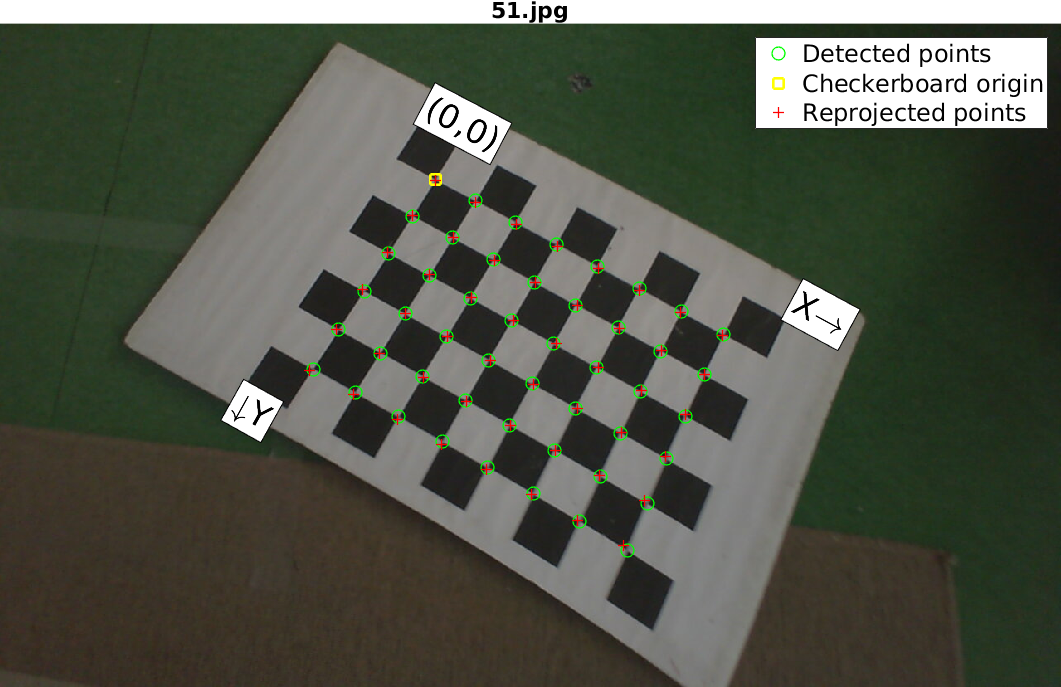
\includegraphics[width=0.7\textwidth]{graphics/worst.png}
\caption{Calibrated image with the highest amount of pixel error}
\label{fig:worst-calibrated-image}
\end{center}
\end{figure}
\begin{itemize}
\item The reprojection error is the distance, in pixels, between the detected and the reprojected points.
\item We notice that the pixel at the bottom-right has the worst reprojection error.
\item This is due to barrel distortion which are slightly inaccurately corrected.
\item The reason for bad distortion calibration is due to the fact that our calibration image set does not include images in which the angle between optical axis of camera and checker board is very high.
\end{itemize}



\begin{figure}[H]
	\centering
	\begin{subfigure}[b]{0.45\textwidth}
		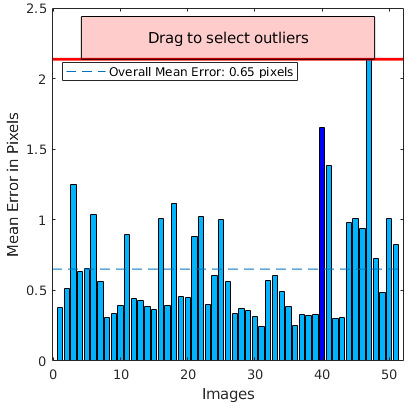
\includegraphics[width=\textwidth]{graphics/stats.png}
		\caption{Mean reprojection error in Pixels for each image.}
		\label{fig:stats}
	\end{subfigure}
	\qquad
	\begin{subfigure}[b]{0.45\textwidth}
		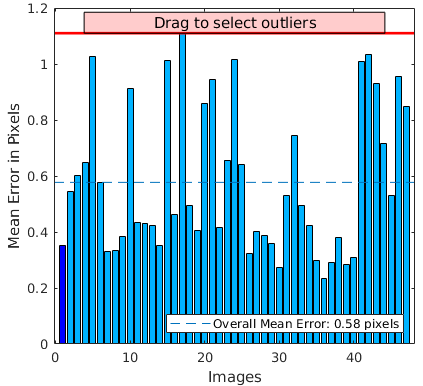
\includegraphics[width=\textwidth]{graphics/stats_improved.png}
		\caption{Mean reprojection error in Pixels for each image after deleting the outliers.}
		\label{fig:statsimproved}
	\end{subfigure}
\end{figure}


\begin{itemize}
\item The mean error (in pixels) per intersection is shown in fig. \ref{fig:stats}.
\item We notice that the mean deviation from the target intersection point is 0.65 pixels which is in sub-pixel regime.
\item After deleting images 11, 45, 46 and 51 which had high reprojection error as shown in fig. \ref{fig:statsimproved}, we observe that mean error (in pixels) per intersection is 0.58 pixels.
\end{itemize}
\subsection{Provide arguments for which camera model best fits your situation and hence should be used.}
\begin{itemize}
\item For our purpose, after disabling auto-focussing, the pin-hole camera model fits our situation best.
\item Pin hole cameras have an extremely tiny aperture and therefore a very wide depth of field. Given the task of pose estimation, wide depth of field is necessary as we can estimate the pose of the object placed at wide range of depth with allowable error.
\item Barrel and pin cushion distortion model is used because it is the most common lens distortion model found in nearly-thin lenses. It allows us to estimate the pose of object placed at wide angle.
\item Mono-chromatic distortion (individual distortion associated with each wavelength) is not considered while calibrating as we will use only gray-scale image.    
\end{itemize}

\subsection{Discuss possible problems or error sources that can disturb the calibration process.}
\begin{itemize}
\item If the calibration images set does not contain diverse enough poses of checker board with respect to camera, we would have higher calibration error.
\item Low brightness setting for experiment that makes detection of checker board intersections harder would also result in low accuracy in calibration.
\item Bad focus can also be the source or errors.
\item Lens distortion is another source of error which has been elaborated further up.
\item Inaccurate measurement of checkerboard side can lead to considerable error which might force us to recalibrate the camera. 
\item Uneven surface of the checkerboard (due to air bubbles) is also a source of error. 
\item Corner estimation, due to above mentioned reasons along with human error can lead to possible error in calibration, but this error will be small because of quantity of images used. 
\item Calibrating camera with lower resolution images can lead to errors if the same results are used to process higher resolution images. 
   
\end{itemize}


%%%%%%%%%%%%%%%%%%%%%%%%%%%%%%%%%%%%%%%%%%%%%%%%%%%%%%%%%%%%%%%%%%%%%%%%%%%%%